\documentclass[12pt,letterpaper]{exam}
\usepackage[lmargin=1in,rmargin=1in,tmargin=1in,bmargin=1in]{geometry}
\usepackage{../style/exams}

% -------------------
% Course & Exam Information
% -------------------
\newcommand{\course}{MATH 141: Final Exam}
\newcommand{\term}{Fall --- 2024}
\newcommand{\examdate}{12/09/2024}
\newcommand{\timelimit}{150 Minutes}

\setbool{hideans}{true} % Student: True; Instructor: False

% -------------------
% Content
% -------------------
\begin{document}

\examtitle
\instructions{Write your name on the appropriate line on the exam cover sheet. This exam contains \numpages\ pages (including this cover page) and \numquestions\ questions. Check that you have every page of the exam. Answer the questions in the spaces provided on the question sheets. Be sure to answer every part of each question and show all your work. If you run out of room for an answer, continue on the back of the page --- being sure to indicate the problem number.} 
\scores
\bottomline
\newpage


% Poem
\phantom{.} \vfill
	\begin{table}[h]
	\centering
	\begin{tabular}{l}
	{\itshape 'Twas the night before Christmas, up at the Pole,} \\
	{\itshape Santa was frazzled---he'd lost all control!} \\
	{\itshape The reindeer were restless, the sleight off its track,} \\
	{\itshape And the toy distribution? A logistical smack!} \\
	\\
	{\itshape Santa scratched his beard, eyes weary and red,} \\
	{\itshape ``The math here is tricky. I'm in over my head!} \\
	{\itshape The children are waiting, and I need to take flight.} \\
	{\itshape I need a Calculus wizard to save Christmas tonight!''}
	\end{tabular}
	\end{table}
\phantom{.} \vfill 

% -------------------
% Questions
% -------------------
\begin{questions}

% Question 1
\newpage
\question[15] {\itshape Santa missing Christmas would be a great crime, \par \phantom{(XX points)} ``Help me dear students, before I run out of time!} \par\vspace{0.3cm}

Showing all your work and using any method, compute the following limits: \par\vspace{0.2cm}
	\begin{enumerate}[(a)]
	\item $\ds\lim_{x \to 2} \dfrac{x^2 + x - 6}{x - 2}$ \vfill
	\item $\ds\lim_{h \to 0} \dfrac{3 - \sqrt{h + 9}}{h}$ \vfill
	\item $\ds\lim_{a \to 0} \dfrac{3a}{\sin(4a)}$ \vfill
	
	\newpage
	
	\item $\ds\lim_{b \to \infty} \left(1 + \dfrac{2}{b} \right)^b$ \vfill
	\item $\ds\lim_{y \to \infty} \dfrac{3y^2 - 4y + 9}{6y^2 + 5y - 1}$ \vfill
	\end{enumerate}



% Question 2
\newpage
\question[15] {\itshape Rudolph's math looked quite queer, and Santa's in doubt. \par \phantom{(XX points)} ``Did you check the derivative? Help me figure it out!''} \par\vspace{0.3cm}

Use the definition of the derivative to find $f'(x)$, where $f(x)= 2x - 3x^2$. You may \textit{\textbf{not}} use derivative shortcuts to find $f'(x)$. \textit{\textbf{Do not}} use l'H\^opital's rule to compute any limits.



% Question 3
\newpage
\question[15] {\itshape Santa's sleigh is on point, but his math's in a tizz, \par \phantom{(XX points)} ``Quick, take these derivatives---I can't lose my rizz!''} \par\vspace{0.3cm}

Showing all your work, compute the following derivatives---\textit{do not simplify your results}:
	\begin{enumerate}[(a)]
	\item $\dfrac{d}{dx} \big( \log_6(x) - \arcsin x + \sec x \big)=$ \vfill
	\item $\dfrac{d}{dx} \left(x^5 \, 2^x \ln x \right)=$ \vfill
	\item $\dfrac{d}{dx}\, \sin^2(1 - e^x)=$ \vfill
	\item $\dfrac{d}{dx} \left( \dfrac{x - \tan^{-1} x}{1 + \cos x} \right)=$ \vfill
	\end{enumerate}



% Question 4
\newpage
\question[15] {\itshape Santa's sleigh is in motion, but the curve's hard to trace, \par \phantom{(XX points)} ``Find the tangent for me---I'm racing through space!''} \par\vspace{0.3cm}

Consider the curve $\mathcal{C}$ given by $xy + y^2= 6$. Showing all your work, find the tangent line to $\mathcal{C}$ at the point $(5, 1)$.



% Question 5
\newpage
\question[15] {\itshape Oh no, Elone has taken to Y---mischief his goal, \par \phantom{(XX points)} But Santa saw through it and stuffed his stocking with coal.} \par\vspace{0.3cm}

Elone fires a missile at Santa in retaliation as Santa flies overhead. At this instant, Santa is 8 miles due south of Elone’s SpaceY base, traveling directly south at 70 mph. The missile, having missed, is 6 miles due east of the base, traveling eastward at 60 mph. How fast is the distance between Santa and the missile changing at this moment?



% Question 6
\newpage
\question[15] {\itshape Santa's workshop is booming, but expenses are a fright. \par \phantom{(XX points)} ``Help me minimize costs, or I'm bankrupt tonight!''} \par\vspace{0.3cm}

A rectangular gift shipping container must have an open top and a volume of 450~cubic meters. The container must also be three times as long as it is wide. Through Christmas magic, the cost of materials for the base is \$1 per square meter, while the material for the sides costs \$2 per square meter. Showing all your work, find the dimensions of the shipping container having minimal cost. {\itshape You do not need to prove that your dimensions give the minimum cost.}



% Question 7
\newpage
\question[15] {\itshape Stuck on a slope, the math's in a twist, \par \phantom{(XX points)} ``Help me analyze the derivative or gifts will be missed!''} \par\vspace{0.3cm}

Below is the plot of the \textit{\textbf{derivative of a function, $f'(x)$}}. {\bfseries This is \textit{not} the graph of $f(x)$.} 
	\[
	\fbox{
	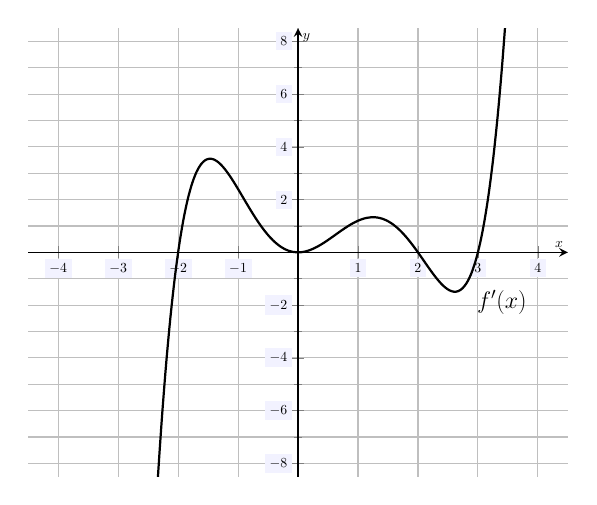
\begin{tikzpicture}[scale=1,every node/.style={scale=0.5}]
	\begin{axis}[
	grid=both,
	axis lines=middle,
	ticklabel style= {fill= blue!5!white},
	xmin= -4.5, xmax=4.5,
	ymin= -8.5, ymax=8.5,
	xtick= {-5,-4,...,5},
	ytick= {-8,-6,...,8},
	minor tick = {-10,-9,...,10},
	xlabel= \(x\), ylabel= \(y\)
	]
	\node at (3.4,-1.9) {\LARGE$f'(x)$};
	\addplot[thick, samples=100, smooth, domain= -3:4.2] ({x},{1/5*x^2*(x + 2)*(x - 2)*(x - 3)});
	\end{axis}
	\end{tikzpicture}
	}
	\]
Based on the plot above, answer the following:
	\begin{enumerate}[(a)]
	\item Identify the intervals where $f(x)$ is increasing and decreasing. \vfill
	\item Classify the $x$-values of any local maxima or local minima for $f(x)$. \vfill
	\item Is $f(x)$ concave up, down, or neither on the interval $(0, 1)$? Justify your answer. \vfill
	\end{enumerate}



% Question 8
\newpage
\question[15] {\itshape Addressing Christmas challenges, Santa has another request. \par \phantom{(XX points)} ``Help me solve this problem---then we'll pass this tough test!''} \par\vspace{0.3cm}

Let $\displaystyle g(x)= \int_0^x f(t) \;dt$, where $f(t)$ is the function whose graph on the interval $[0, 9]$ is shown below. 
	\[
	\fbox{
	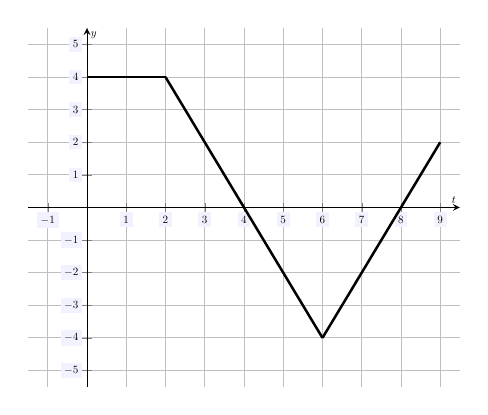
\begin{tikzpicture}[scale=0.8,every node/.style={scale=0.5}]
	\begin{axis}[
	grid=both,
	axis lines=middle,
	ticklabel style= {fill= blue!5!white},
	xmin= -1.5, xmax=9.5,
	ymin= -5.5, ymax=5.5,
	xtick= {-2,-1,...,10},
	ytick= {-6,-5,...,6},
	minor tick = {-10,-9,...,10},
	xlabel= \(t\), ylabel= \(y\)
	]
	\addplot[line width=0.04cm, samples=4, smooth, domain= 0:2] {4};
	\addplot[line width=0.04cm, samples=4, smooth, domain= 2:6] {8 - 2*x};
	\addplot[line width=0.04cm, samples=4, smooth, domain= 6:9] {2*x - 16};
	
	\end{axis}
	\end{tikzpicture}
	}
	\] 

\begin{enumerate}[(a)]
\item Showing all your work, compute $g(8)$. \vfill
\item On what interval(s) is $g(x)$ decreasing? Justify your answer. \vfill
\item Find and classify any local minima/maxima for $g(x)$. Justify your answer. \vfill
\item Showing all your work, compute $g''(4)$. \vfill
\end{enumerate}



% Question 9
\newpage
\question[15] {\itshape Snow's on the way, and Santa's on a tight schedule today. \par\phantom{(XX points)} Find the maxima and minima, there's no time to---you know what? \par \phantom{(XX points)} Don't question Santa. Just find the maxima and minima.} \par\vspace{0.3cm}

Let $f(x)= 2x - 3x^{2/3}$. Showing all your work, find the absolute maxima and minima of $f(x)$ on the interval $[-1, 3]$. Be sure to justify your answers with an appropriate derivative test. 



% Question 10
\newpage
\question[15] {\itshape Christmas almost over, you're nearly clear. \par \phantom{(XX points)} ``Help me find these integrals, then we're done for this year.''} \par\vspace{0.3cm}

Showing all your work, compute the following: \par\vspace{0.2cm}
	\begin{enumerate}[(a)]
	\item $\ds\int \left( \sin x - e^x + \dfrac{1}{x^2 + 1} \right) dx$ \vfill
	\item $\ds\int_1^2 \left( \dfrac{1 - x}{x} \right)^2 dx$ \vfill
	
	\newpage
	
	\item $\ds\int \dfrac{dx}{x \ln x}$ \vfill
	\item $\ds\int_0^{\pi/2} \cos^3(x) \sin(x) \;dx$ \vfill
	\end{enumerate}

\end{questions}


% End Poem
\newpage

\phantom{.} \vfill
	\begin{table}[h]
	\centering
	\begin{tabular}{l}
	{\itshape Santa exclaimed, at the end of Christmas night,} \\
	{\itshape ``Thanks to you, the math's worked out right!} \\
	{\itshape Stay curious, dear student, keeping Mathematics in sight,} \\
	{\itshape And merry Christmas to all, and to all a good night!}
	\end{tabular}
	\end{table}
\phantom{.} \vfill

\end{document}